\chapter{Análisis}

\section{Introducción}

Para abordar cualquier proyecto que se desee desarrollar, debe ser sometido a un infructuoso proceso de análisis, y esto se debe principalmente a que es imposible empezar una construcción sin tener unos planos, que ayuden como guía en el proceso, no solo de hacer una construcción, sino asegurando que sea un desarrollo robusto, y además que asegure un mantenimiento posterior.

Es por esto que en el presente capítulo, se dedicará a describir el análisis de cada requerimiento, mostrando el proceso en cada aspecto tratado en nuestro proyecto.

\section{Diagrama de Casos de Uso}

\begin{figure}[h!]
	\centering
	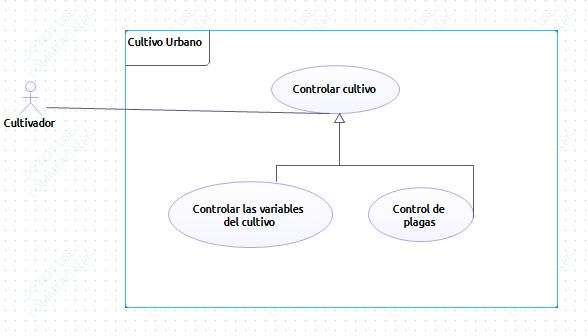
\includegraphics[width=1.2\linewidth]{proyecto/imgs/Caso de uso}
	\caption{Diagrama de Casos de Uso}
	\label{fig:cronograma}
\end{figure}


\subsection{Requerimientos Específicos}


\begin{table}[]
	\centering
	\caption{Requerimiento específico del riego del cultivo.}
	\label{my-label}
	\begin{tabular}{|
			>{\columncolor[HTML]{7BD4EE}}c |c|c|}
		\hline
		{\color[HTML]{000000} \textbf{Nombre}}                   & Riego del cultivo                                                         & ID : 1                                                       \\ \hline
		{\color[HTML]{000000} \textbf{Objetivo}}                 & \multicolumn{2}{c|}{\begin{tabular}[c]{@{}c@{}}Controlar y medir la cantidad\\  de agua suministrada a las plantas\end{tabular}}         \\ \hline
		{\color[HTML]{000000} \textbf{Actores}}                  & \multicolumn{2}{c|}{Cultivador}                                                                                                          \\ \hline
		{\color[HTML]{000000} \textbf{Escenario Primario}}       & \multicolumn{2}{c|}{Se hace el riego de manera exitosa}                                                                                  \\ \hline
		{\color[HTML]{000000} \textbf{Escenario Secundario}}     & \multicolumn{2}{c|}{\begin{tabular}[c]{@{}c@{}}El riego no se lleva a cabo de\\  manera exitosa. (Exceso y Deficit)\end{tabular}}        \\ \hline
		{\color[HTML]{000000} \textbf{Escenarios Excepcionales}} & \multicolumn{2}{c|}{\begin{tabular}[c]{@{}c@{}}- No se dispone de agua .\\ - El sistema de riego no funciona. \\ - Lluvias\end{tabular}} \\ \hline
	\end{tabular}
\end{table}


\begin{table}[]
	\centering
	\caption{My caption}
	\label{my-label}
	\begin{tabular}{|
			>{\columncolor[HTML]{7BD4EE}}c |c|c|}
		\hline
		{\color[HTML]{000000} \textbf{Nombre}}                   & Iluminación del cultivo                                                                                 & ID : 2                                                                                \\ \hline
		{\color[HTML]{000000} \textbf{Objetivo}}                 & \multicolumn{2}{c|}{\begin{tabular}[c]{@{}c@{}}Controlar la cantidad e intensidad de\\ luminosidad que recibe el cultivo\end{tabular}}                                                          \\ \hline
		{\color[HTML]{000000} \textbf{Actores}}                  & \multicolumn{2}{c|}{Cultivador}                                                                                                                                                                 \\ \hline
		{\color[HTML]{000000} \textbf{Escenario Primario}}       & \multicolumn{2}{c|}{\begin{tabular}[c]{@{}c@{}}El cultivo recibe la cantidad de luz\\  necesaria que garantice su crecimiento \\ óptimo\end{tabular}}                                           \\ \hline
		{\color[HTML]{000000} \textbf{Escenario Secundario}}     & \multicolumn{2}{c|}{\begin{tabular}[c]{@{}c@{}}La luz solar se incrementa a causa \\ de un verano y sequía\end{tabular}}                                                                        \\ \hline
		{\color[HTML]{000000} \textbf{Escenarios Excepcionales}} & \multicolumn{2}{c|}{\begin{tabular}[c]{@{}c@{}}- El sistema que brinda \\ luz y sombra al\\  cultivo deja de funcionar\\ -Obstáculos externos que impidan\\ la llegada de la luz.\end{tabular}} \\ \hline
	\end{tabular}
\end{table}


\begin{table}[]
	\centering
	\caption{Requerimiento específico del pH del cultivo}
	\label{my-label}
	\begin{tabular}{|
			>{\columncolor[HTML]{7BD4EE}}c |c|c|}
		\hline
		{\color[HTML]{000000} \textbf{Nombre}}                   & Estabilidad del Ph del cultivo                                                                  & ID : 3                                                                \\ \hline
		{\color[HTML]{000000} \textbf{Objetivo}}                 & \multicolumn{2}{c|}{\begin{tabular}[c]{@{}c@{}}Controlar y estabilizar el nivel de  pH  \\ de la tierra usada en el cultivo\end{tabular}}                               \\ \hline
		{\color[HTML]{000000} \textbf{Actores}}                  & \multicolumn{2}{c|}{Cultivador}                                                                                                                                         \\ \hline
		{\color[HTML]{000000} \textbf{Escenario Primario}}       & \multicolumn{2}{c|}{\begin{tabular}[c]{@{}c@{}}El cultivo tiene el pH adecuado \\ para el optimo crecimiento \\ de la planta dependiendo de su tipo.\end{tabular}}      \\ \hline
		{\color[HTML]{000000} \textbf{Escenario Secundario}}     & \multicolumn{2}{c|}{}                                                                                                                                                   \\ \hline
		{\color[HTML]{000000} \textbf{Escenarios Excepcionales}} & \multicolumn{2}{c|}{\begin{tabular}[c]{@{}c@{}}El nivel del pH es bajo debido a : \\ -Nivel de fertilización del cultivo\\ -Lluvias Ácidas\\ -Entre otras\end{tabular}} \\ \hline
	\end{tabular}
\end{table}

\newpage

\subsection{Diagrama de Secuencia}

\newpage

\subsection{Diagrama de Comunicación}

\newpage

\subsection{Diagrama de Temporización}

\newpage

\section{Diagramas de Actividades}

\newpage

\section{Diagramas de Actividades}

\newpage

\section{Diagramas de Workflow}

\newpage

\section{Diagramas de Descripción de la Interacción}

\newpage